\documentclass[12pt,a4paper]{article}

\usepackage[utf8]{inputenc}
\usepackage[margin=1in]{geometry}
\usepackage{graphicx}
\usepackage{float}
\usepackage{amsmath}
\usepackage{amssymb}
\usepackage{booktabs}
\usepackage{hyperref}
\usepackage{listings}
\usepackage{xcolor}
\usepackage{caption}
\usepackage{enumitem}
\usepackage{fancyhdr}

% Code listing style
\lstdefinestyle{verilog}{
    language=Verilog,
    basicstyle=\ttfamily\footnotesize,
    keywordstyle=\color{blue}\bfseries,
    commentstyle=\color{green!50!black},
    stringstyle=\color{red},
    numbers=left,
    numberstyle=\tiny\color{gray},
    numbersep=5pt,
    frame=single,
    breaklines=true,
    tabsize=4,
    showstringspaces=false
}

\lstdefinestyle{xdc}{
    basicstyle=\ttfamily\footnotesize,
    keywordstyle=\color{blue}\bfseries,
    commentstyle=\color{green!50!black},
    numbers=left,
    numberstyle=\tiny\color{gray},
    numbersep=5pt,
    frame=single,
    breaklines=true,
    tabsize=4,
    showstringspaces=false
}

\pagestyle{fancy}
\fancyhf{}
\rhead{FPGA Lab -- Experiment 3}
\lhead{Tel Aviv University}
\cfoot{\thepage}

\begin{document}

% ============================================================
% TITLE PAGE
% ============================================================
\begin{titlepage}
    \centering
    \vspace*{2cm}
    {\LARGE \textbf{FPGA Experiment Report} \par}
    \vspace{1cm}
    {\Large Task: FPGA 3 -- 7 Segment and LEDs \par}
    \vspace{2cm}
    {\large
    \begin{tabular}{ll}
        \textbf{Student 1:} & Name: \underline{\hspace{4cm}} \quad ID: \underline{\hspace{3cm}} \\[10pt]
        \textbf{Student 2:} & Name: \underline{\hspace{4cm}} \quad ID: \underline{\hspace{3cm}} \\
    \end{tabular}
    \par}
    \vspace{2cm}
    {\large Tel Aviv University \\
    The Iby and Aladar Fleischman Faculty of Engineering \\
    FPGA Laboratory \par}
    \vfill
\end{titlepage}

% ============================================================
% PART 1 -- STATUS UPDATE
% ============================================================
\section*{Part 1 -- Status Update}

Fill in the following table according to your progress at the time of the submission.
Each row should refer to one of the modules together with its simulation.

The status column should be filled with one of the following:
\begin{itemize}[nosep]
    \item \textbf{Done} -- If both are written and simulation passed.
    \item \textbf{Partially done} -- If you started writing the module and simulation but it's not working properly.
    \item \textbf{Not started} -- If you didn't get to that part of the task.
\end{itemize}

When the status is partially done, please use the notes/comments column to explain in a few more words what is the status of the module and what is the status of the simulation.

\vspace{0.5cm}
\begin{table}[H]
    \centering
    \begin{tabular}{|l|c|l|}
        \hline
        \textbf{Module name/Step} & \textbf{Status} & \textbf{Notes/Comments} \\
        \hline
        Seven Segment Display     & Done             &                          \\
        \hline
        Display Playground        & Done             &                          \\
        \hline
        Setting up constraints    & Done             &                          \\
        \hline
        Implementing the design   & Done             &                          \\
        \hline
    \end{tabular}
\end{table}

\subsection*{Issues}
In this section please describe the current issues you are facing.

\begin{itemize}[nosep]
    \item Seven Segment Display: No issues.
    \item Display Playground: No issues.
    \item Setting up constraints: No issues.
    \item Implementing the design: No issues.
\end{itemize}

\newpage
% ============================================================
% PART 2 -- SIMULATIONS AND ANSWERS
% ============================================================
\section*{Part 2 -- Simulations and Answers}

% ------------------------------------------------------------
% SECTION 2: SEVEN SEGMENT DISPLAY
% ------------------------------------------------------------
\subsection*{Seven Segment Display}

\subsubsection*{2c. Refresh Frequency Selection}

The BASYS3 board uses a 100~MHz clock, so the clock period is $T_{clk} = 10$~ns.
Inside the \texttt{Seg\_7\_Display} module, a 20-bit counter \texttt{clkdiv} increments on every rising clock edge.
The least significant bit (LSB) toggles every 10~ns, and in general, the $n$-th bit toggles every $10 \times 2^{n}$~ns.

According to the experiment instructions, the total refresh time for all 4 digits must be between 1~ms and 16~ms. Since there are four digits, we need two bits from the counter to cycle through them (values 00, 01, 10, 11).

We chose:
\[
s = \texttt{clkdiv}[19:18]
\]

Each digit selection changes every $10 \times 2^{18}$~ns $= 2.62$~ms. For all four digits, the total refresh period is:
\[
T_{refresh} = 4 \times 2.62~\text{ms} = 10.49~\text{ms}
\]

This satisfies the requirement $1~\text{ms} \leq T_{refresh} \leq 16~\text{ms}$, ensuring flicker-free display for the human eye.

\newpage
% ------------------------------------------------------------
% SECTION 3: DISPLAY PLAYGROUND
% ------------------------------------------------------------
\subsection*{Display Playground}

\subsubsection*{3b. Block Diagram}

The Display Playground module architecture consists of the following functional blocks:

\begin{itemize}[nosep]
    \item \textbf{Input clamping logic:} Four parallel comparators check whether each 4-bit switch group (\texttt{sw[3:0]}, \texttt{sw[7:4]}, \texttt{sw[11:8]}, \texttt{sw[15:12]}) exceeds the value 9. If so, a multiplexer replaces the value with 9 (4'b1001). Otherwise the original switch value passes through.
    \item \textbf{Seg\_7\_Display instance:} The clamped 16-bit value \texttt{fixed\_sw} is fed to the \texttt{Seg\_7\_Display} module, which handles the time-multiplexed driving of the four 7-segment digits.
    \item \textbf{LED decoder:} A case statement maps the first digit (\texttt{fixed\_sw[3:0]}) to the corresponding LED (0--9), producing a one-hot encoding on the 10 LEDs.
\end{itemize}

\begin{figure}[H]
    \centering
    \fbox{\parbox{0.9\textwidth}{
    \centering
    \vspace{0.3cm}
    \textbf{Block Diagram of Display\_Playground}\\[0.3cm]
    \texttt{sw[15:0]} $\rightarrow$ \fbox{Clamp ($>$9 $\rightarrow$ 9)} $\rightarrow$ \texttt{fixed\_sw[15:0]} $\rightarrow$ \fbox{Seg\_7\_Display} $\rightarrow$ \texttt{seg[6:0], an[3:0], dp}\\[0.3cm]
    \hspace{5.5cm} \texttt{fixed\_sw[3:0]} $\rightarrow$ \fbox{LED Case Decoder} $\rightarrow$ \texttt{led[9:0]}\\[0.3cm]
    \texttt{clk} $\rightarrow$ \fbox{Seg\_7\_Display}
    \vspace{0.3cm}
    }}
    \caption{Simplified block diagram of the Display\_Playground module.}
\end{figure}

\subsubsection*{3c. Behavior for Invalid Switch Values}

If the switches indicate a number greater than 9 (for example, \texttt{4'b1101} which equals 13 in decimal), the design clamps the value to 9, the maximum single decimal digit. This is implemented using a generate loop with comparators: for each 4-bit group, if the value exceeds \texttt{4'd9}, it is replaced by \texttt{4'd9}. This prevents undefined behavior on the 7-segment display and ensures only digits 0--9 are ever shown.

\subsubsection*{3f. Elaborated Design Schematic}

\begin{figure}[H]
    \centering
    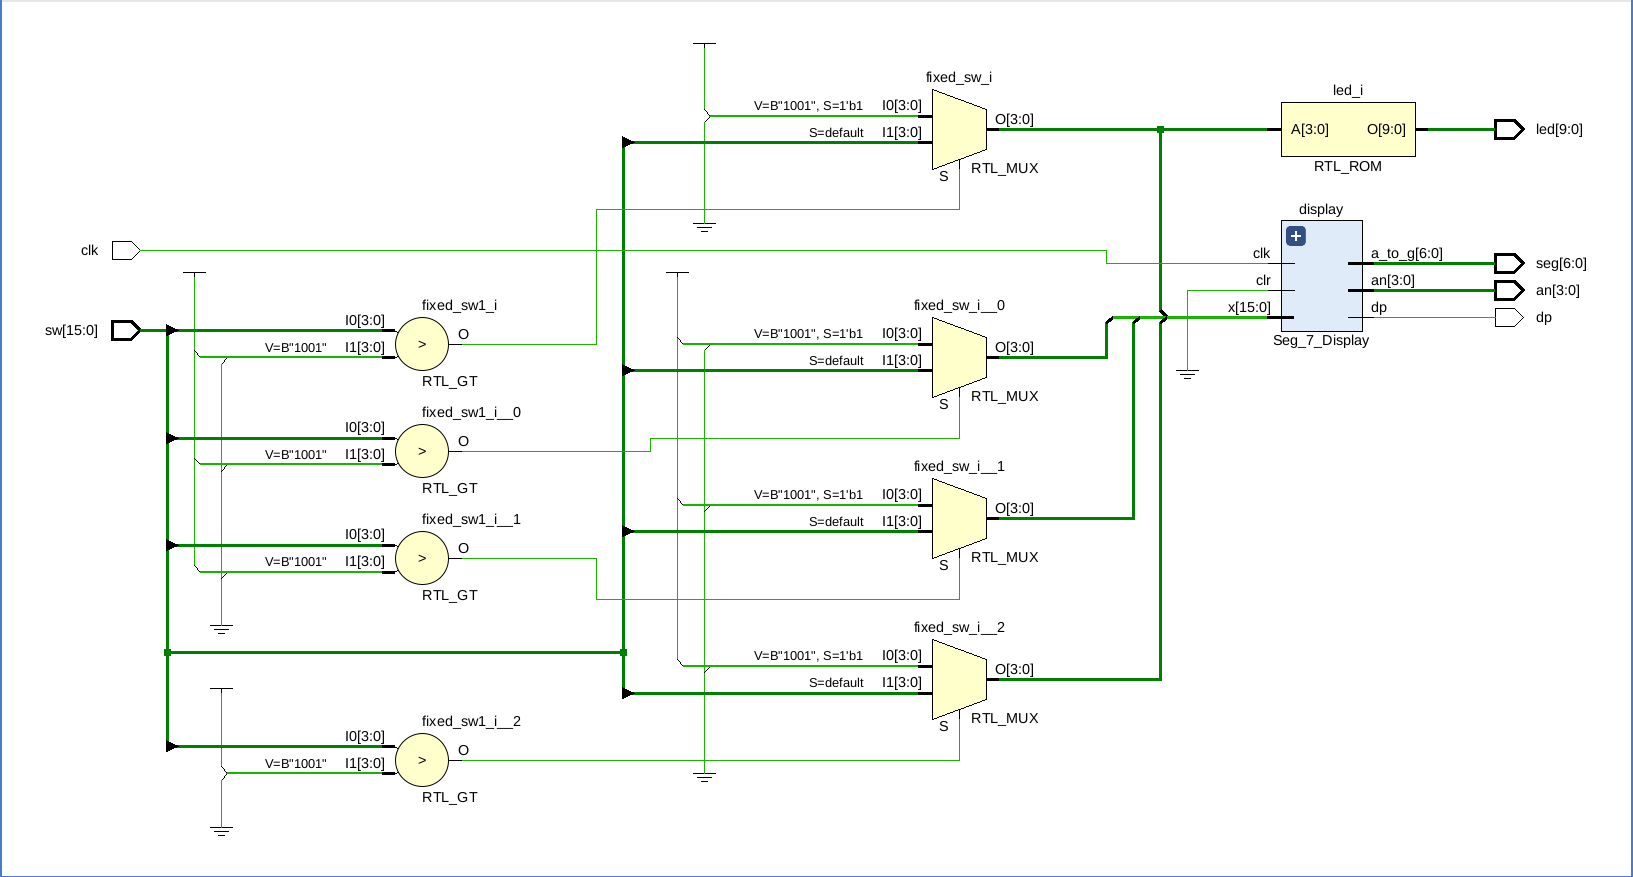
\includegraphics[width=\textwidth]{linter_des.png}
    \caption{RTL elaborated design schematic of Display\_Playground. The schematic shows four \texttt{RTL\_GT} comparators checking each 4-bit switch group against 9, four \texttt{RTL\_MUX} multiplexers selecting between the original and clamped values, an \texttt{RTL\_ROM} for the LED decoder, and the instantiated \texttt{Seg\_7\_Display} module.}
\end{figure}

\subsubsection*{3g. Synthesized Design Schematic}

\begin{figure}[H]
    \centering
    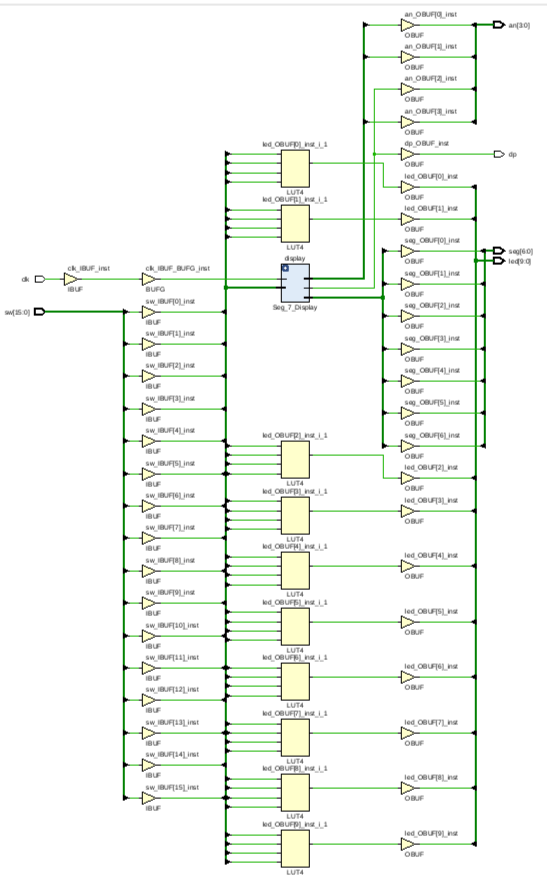
\includegraphics[width=0.65\textwidth]{synthesis_sch.png}
    \caption{Synthesized design schematic of Display\_Playground. The comparators and muxes have been optimized into \texttt{LUT4} look-up tables. Input buffers (\texttt{IBUF}) and output buffers (\texttt{OBUF}) have been inserted for the physical I/O. The clock input passes through a \texttt{BUFG} global clock buffer.}
\end{figure}

In the elaborated design, we see the logical structure of the design as written in Verilog, before any optimization. Modules, registers, and logic blocks are connected exactly as described in the HDL source code.

In the synthesized design schematic, we see the actual hardware resources that the FPGA will use to implement the design. The high-level constructs (comparators, multiplexers, ROM) are mapped to FPGA primitives such as LUT4 look-up tables, and I/O buffer primitives (IBUF, OBUF, BUFG) are inserted for all external connections.

\newpage
% ------------------------------------------------------------
% SECTION 4: SETTING UP CONSTRAINTS
% ------------------------------------------------------------
\subsection*{Setting Up Constraints}

The constraints file \texttt{fpga\_lab\_constraints.xdc} was configured as follows:

\begin{enumerate}[nosep]
    \item \textbf{Clock signal:} Uncommented the two lines connecting \texttt{clk} to pin \texttt{W5} with LVCMOS33 I/O standard.
    \item \textbf{Timing constraint:} Uncommented the \texttt{create\_clock} command specifying a 10~ns period (100~MHz) for \texttt{sys\_clk\_pin}.
    \item \textbf{Switch inputs:} Uncommented all 16 switch lines (\texttt{sw[0]} through \texttt{sw[15]}).
    \item \textbf{7-segment outputs:} Uncommented the 7 segment lines (\texttt{seg[0]}--\texttt{seg[6]}), the 4 anode lines (\texttt{an[0]}--\texttt{an[3]}), and the decimal point (\texttt{dp}).
    \item \textbf{LED outputs:} Uncommented 10 LED output pins (\texttt{led[0]}--\texttt{led[9]}) mapped to pins U16, E19, U19, V19, W18, U15, U14, V14, V13, and V3.
\end{enumerate}

\newpage
% ------------------------------------------------------------
% SECTION 5: IMPLEMENTING THE DESIGN
% ------------------------------------------------------------
\subsection*{Implementing the Design}

\subsubsection*{5c. Implementation Design View}

\begin{figure}[H]
    \centering
    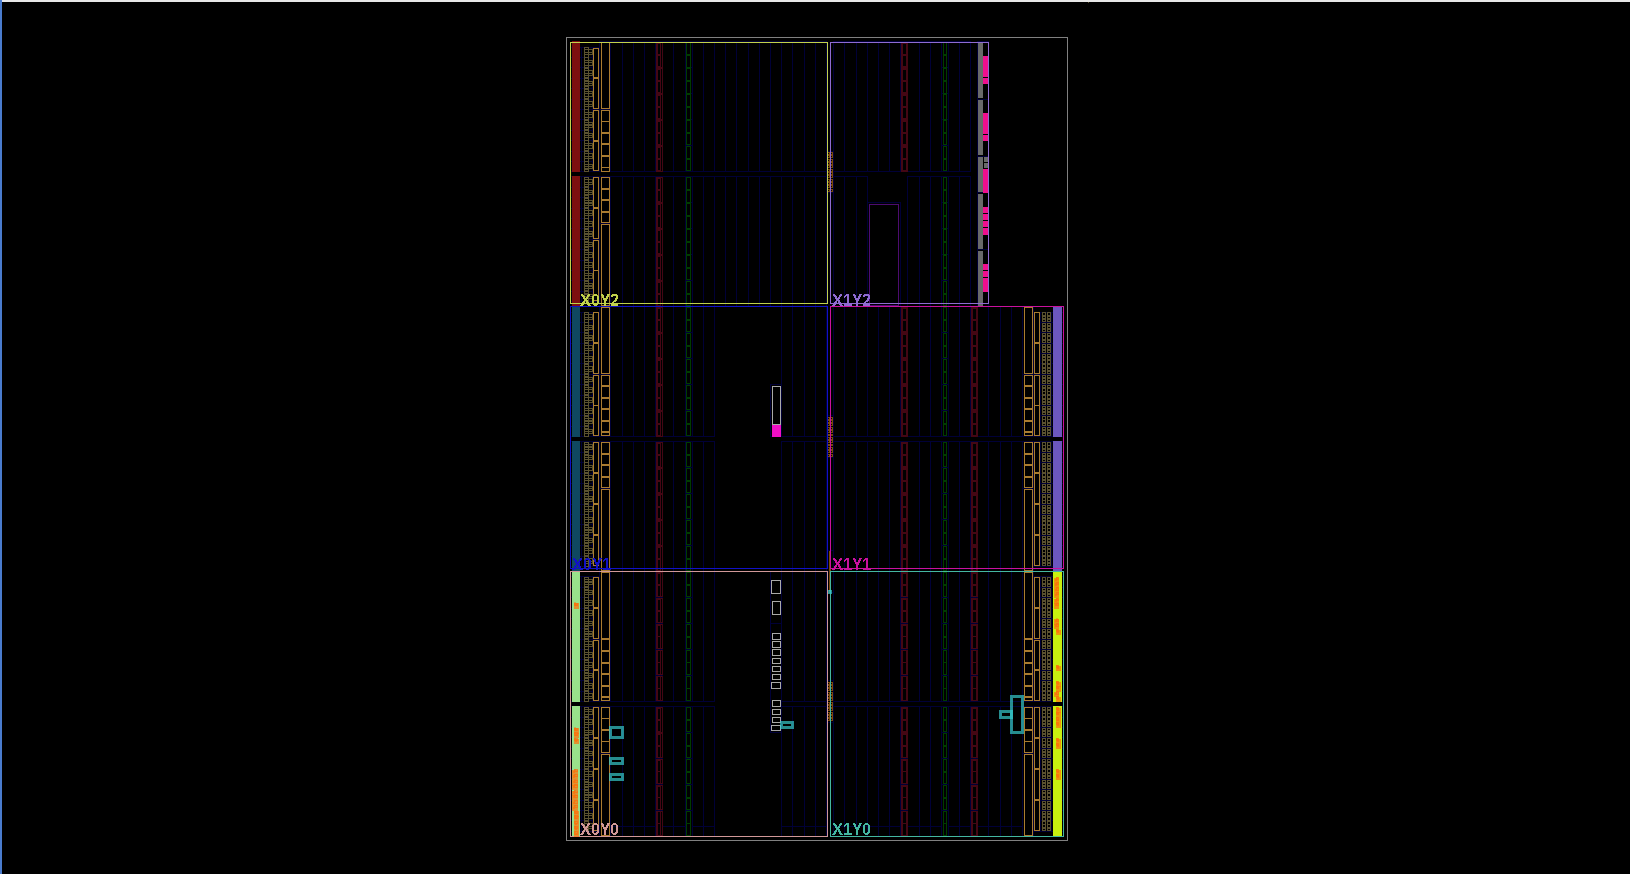
\includegraphics[width=0.8\textwidth]{implemntation_des.png}
    \caption{FPGA implementation floorplan view showing the placed and routed design on the Artix-7 device. The utilized resources are concentrated in a small region of the chip.}
\end{figure}

\subsubsection*{5d. Timing Summary}

\begin{figure}[H]
    \centering
    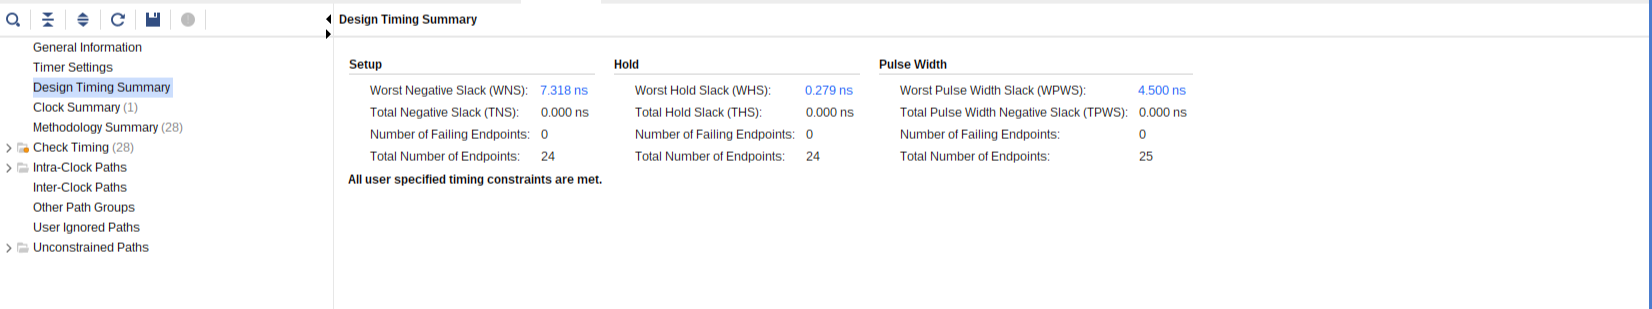
\includegraphics[width=\textwidth]{timing_rep.png}
    \caption{Design Timing Summary showing positive slack for both setup and hold times. All user-specified timing constraints are met.}
\end{figure}

The timing summary confirms:
\begin{itemize}[nosep]
    \item \textbf{Setup:} Worst Negative Slack (WNS) = 7.318~ns (positive $\Rightarrow$ constraint met)
    \item \textbf{Hold:} Worst Hold Slack (WHS) = 0.279~ns (positive $\Rightarrow$ constraint met)
    \item \textbf{Pulse Width:} Worst Pulse Width Slack (WPWS) = 4.500~ns (positive $\Rightarrow$ constraint met)
    \item Number of Failing Endpoints: 0 for all categories
\end{itemize}

\subsubsection*{5e. Critical Setup Path Length}

The critical setup path length can be calculated from the worst negative slack:

\[
\text{setup slack} = T_{clk} - T_{critical\_path}
\]
\[
7.318 = 10 - T_{critical\_path}
\]
\[
T_{critical\_path} = 2.682~\text{ns}
\]

This can be verified from the Vivado timing report:

\begin{figure}[H]
    \centering
    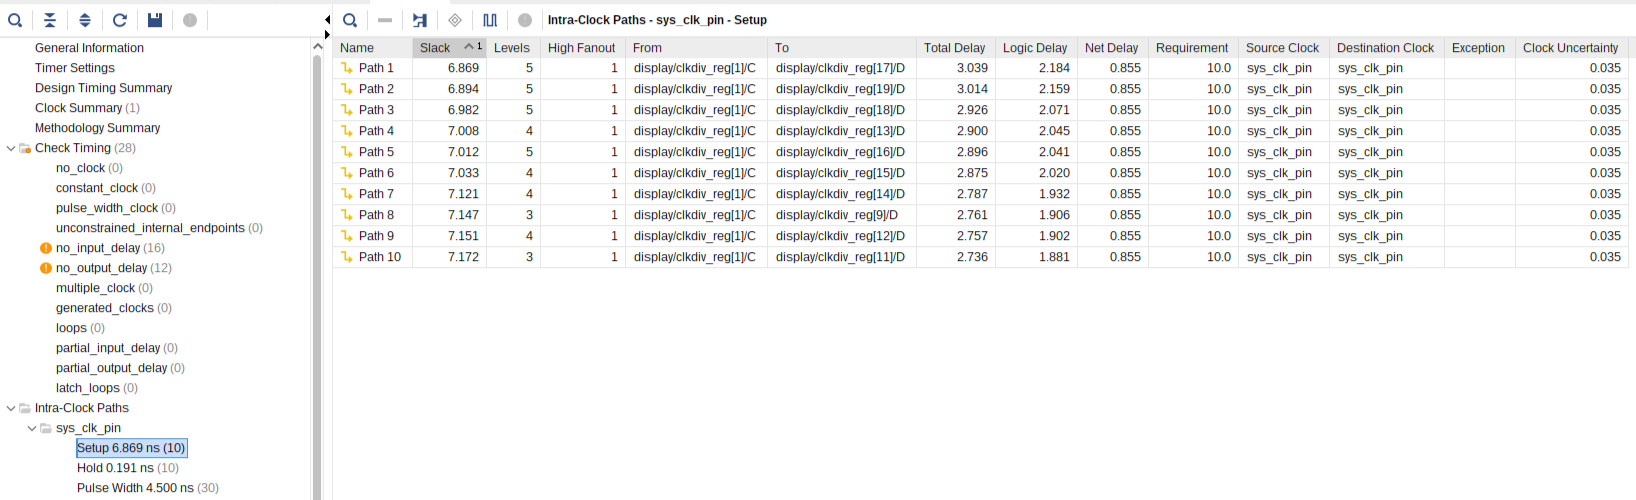
\includegraphics[width=\textwidth]{critical_path.png}
    \caption{Intra-Clock Paths showing the critical path from \texttt{display/clkdiv\_reg[1]/C} to \texttt{display/clkdiv\_reg[17]/D} with a total delay of 3.039~ns and a slack of 6.869~ns.}
\end{figure}

From the Vivado tool, the critical path (Path~1) has a total delay of 3.039~ns, which is consistent with the calculated value. The small difference is due to the inclusion of clock uncertainty (0.035~ns) in the slack computation.

\newpage
% ------------------------------------------------------------
% SECTION 6: FPGA PROGRAMMING
% ------------------------------------------------------------
\subsection*{FPGA Programming}

\subsubsection*{6a--b. Bitstream Generation and Programming}

The bitstream was generated successfully and the design was programmed onto the BASYS3 board.

\begin{figure}[H]
    \centering
    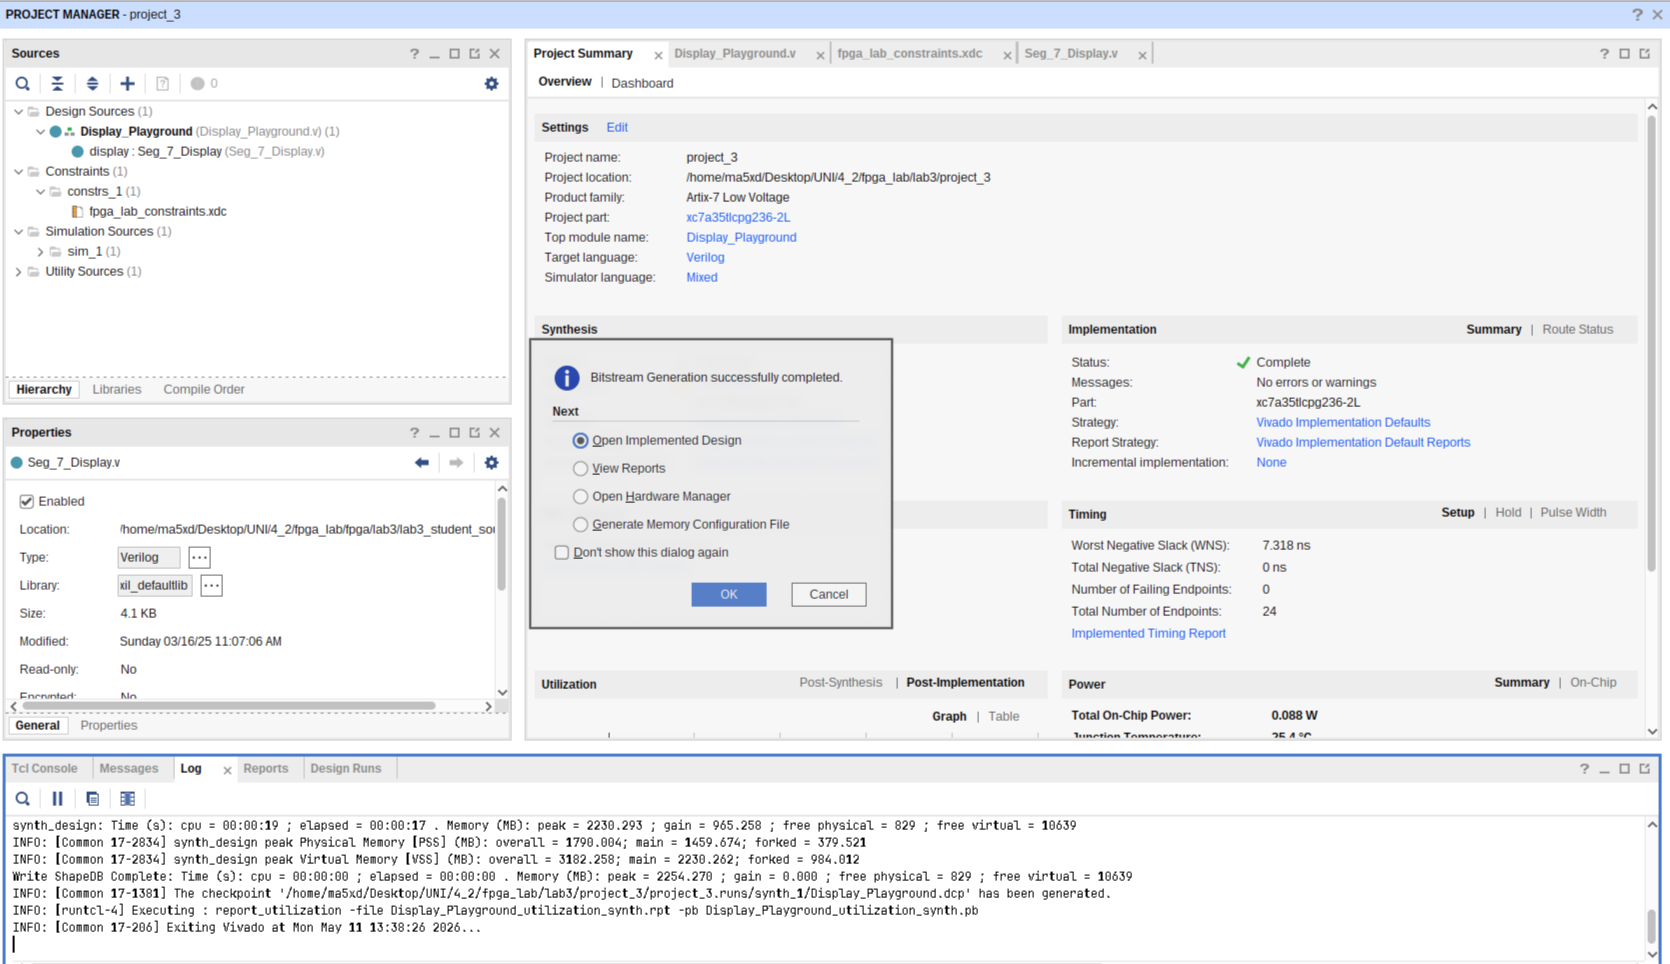
\includegraphics[width=\textwidth]{bit_stream.png}
    \caption{Project Summary showing successful bitstream generation. Implementation status is ``Complete'' with no errors or warnings. WNS = 7.318~ns, Total On-Chip Power = 0.088~W.}
\end{figure}

The design was verified on hardware: setting the 16 switches to represent four decimal digits correctly displayed them on the 7-segment display, and the corresponding LED for the first digit lit up.

\subsubsection*{6c. Post-Implementation Summary (Debug Core Removed)}

After removing the debug core and re-implementing the design:

\begin{figure}[H]
    \centering
    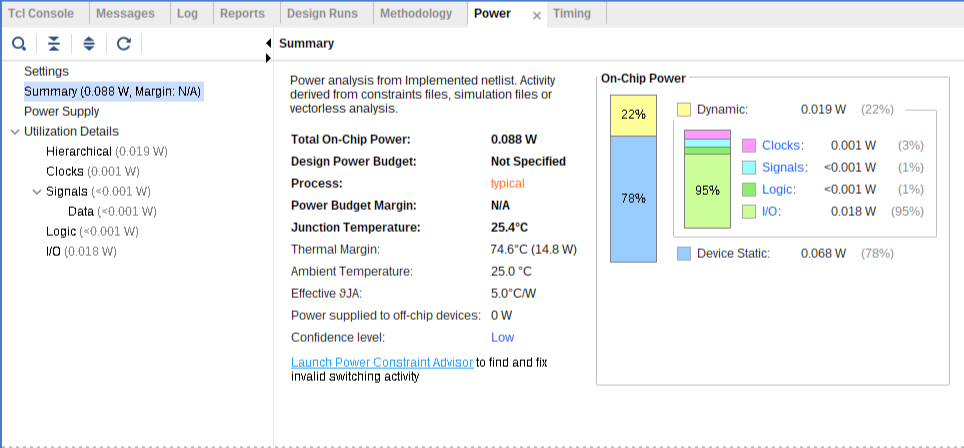
\includegraphics[width=0.85\textwidth]{power_report.png}
    \caption{Power report summary. Total On-Chip Power = 0.088~W, consisting of 0.019~W dynamic (22\%) and 0.068~W static (78\%). Junction temperature = 25.4$^{\circ}$C.}
\end{figure}

\begin{figure}[H]
    \centering
    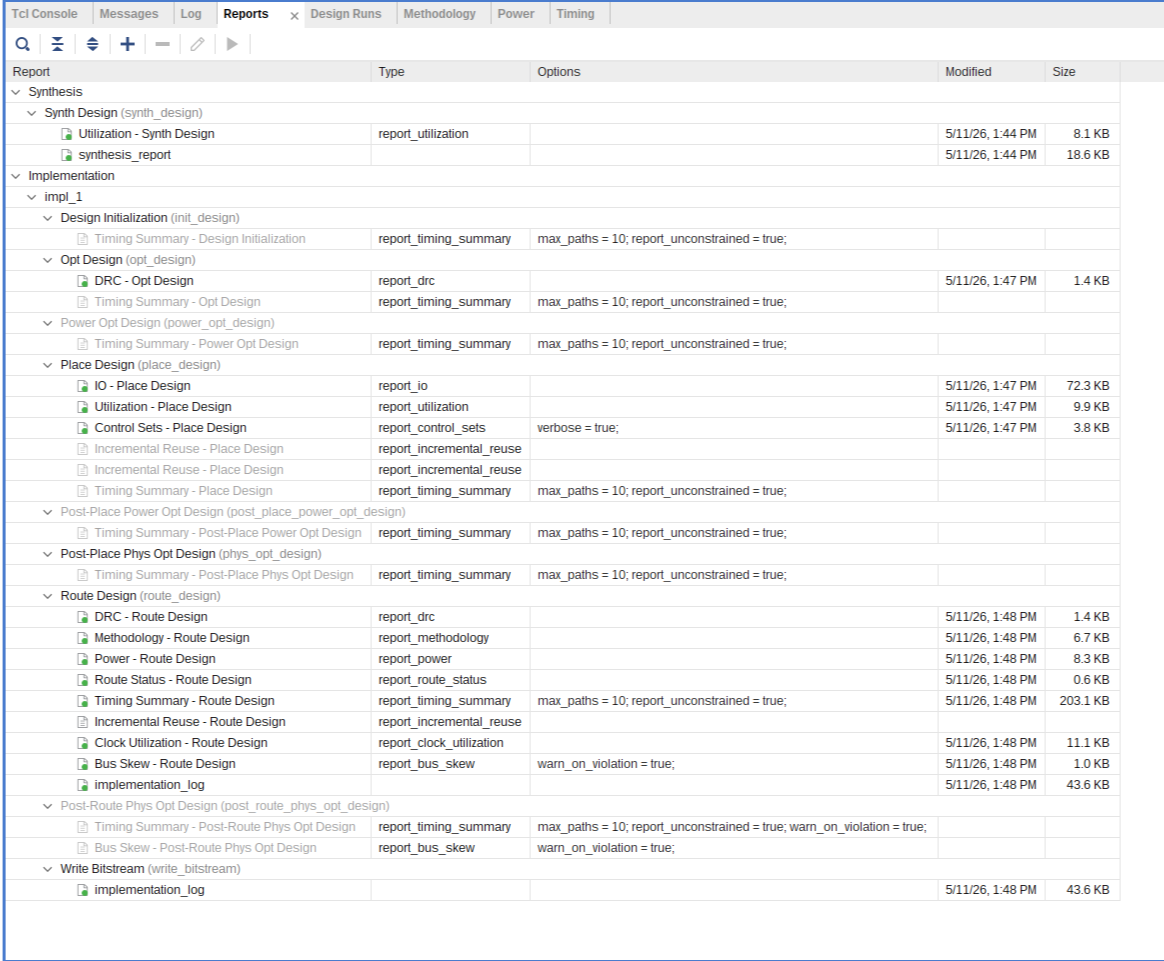
\includegraphics[width=\textwidth]{reports.png}
    \caption{Vivado Reports tab showing all synthesis and implementation reports generated successfully.}
\end{figure}

\newpage
% ------------------------------------------------------------
% APPENDIX: VERILOG SOURCE CODE
% ------------------------------------------------------------
\section*{Appendix A -- Verilog Source Code}

\subsection*{A.1 Seg\_7\_Display.v}
\begin{lstlisting}[style=verilog]
`timescale 1ns/10ps
//////////////////////////////////////////////////////////////
// Company:         Tel Aviv University
// Module Name:     Seg_7_Display
// Description:     Translates input vector "x" into 7-segment
//                  display signals with time-multiplexed digits
//////////////////////////////////////////////////////////////
module Seg_7_Display(
    input [15:0] x,
    input clk,
    input clr,
    output reg [6:0] a_to_g,
    output reg [3:0] an,
    output wire dp
);

    wire [1:0] s;
    reg [3:0] digit;

    // For 100MHz clock
    reg [19:0] clkdiv = 19'b0;
    assign s = clkdiv[19:18];

    assign dp = (s == 2'b10) ? 0 : 1;

    always @(posedge clk)
        case(s)
            0: digit = x[3:0];
            1: digit = x[7:4];
            2: digit = x[11:8];
            3: digit = x[15:12];
            default: digit = x[3:0];
        endcase

    // 7-segment decoder
    always @(*)
        case(digit)
            0:  a_to_g = 7'b1000000;
            1:  a_to_g = 7'b1111001;
            2:  a_to_g = 7'b0100100;
            3:  a_to_g = 7'b0110000;
            4:  a_to_g = 7'b0011001;
            5:  a_to_g = 7'b0010010;
            6:  a_to_g = 7'b0000010;
            7:  a_to_g = 7'b1111000;
            8:  a_to_g = 7'b0000000;
            9:  a_to_g = 7'b0010000;
            'hA: a_to_g = 7'b0111111; // dash
            'hB: a_to_g = 7'b1111111; // off
            'hC: a_to_g = 7'b1110111;
            default: a_to_g = 7'b0000000;
        endcase

    // Anode selection (active low)
    always @(*) begin
        an = 4'b1111;
        an[s] = 0;
    end

    // Clock divider counter
    always @(posedge clk or posedge clr) begin
        if (clr == 1)
            clkdiv <= 0;
        else
            clkdiv <= clkdiv + 1;
    end
endmodule
\end{lstlisting}

\newpage
\subsection*{A.2 Display\_Playground.v}
\begin{lstlisting}[style=verilog]
`timescale 1ns/10ps
//////////////////////////////////////////////////////////////
// Company:         Tel Aviv University
// Module Name:     Display_Playground
// Description:     Top module - switches select display values,
//                  LEDs indicate first digit
// Dependencies:    Seg_7_Display
//////////////////////////////////////////////////////////////
module Display_Playground(clk, sw, seg, an, dp, led);

    input clk;
    input [15:0] sw;
    output wire [6:0] seg;
    output wire [3:0] an;
    output wire       dp;
    output reg [9:0] led;

    reg [15:0] fixed_sw;

    genvar i;
    for (i = 0; i < 4; i = i + 1) begin
        always @(*) begin
            if (sw[(i*4)+3:i*4] > 4'd9)
                fixed_sw[(i*4)+3:i*4] = 4'd9;
            else
                fixed_sw[(i*4)+3:i*4] = sw[(i*4)+3:i*4];
        end
    end

    always @(*) begin
        led = 0;
        case(fixed_sw[3:0])
            4'b0000: led[0] = 1'b1;
            4'b0001: led[1] = 1'b1;
            4'b0010: led[2] = 1'b1;
            4'b0011: led[3] = 1'b1;
            4'b0100: led[4] = 1'b1;
            4'b0101: led[5] = 1'b1;
            4'b0110: led[6] = 1'b1;
            4'b0111: led[7] = 1'b1;
            4'b1000: led[8] = 1'b1;
            4'b1001: led[9] = 1'b1;
            default: led = 0;
        endcase
    end

    Seg_7_Display display(fixed_sw, clk, 0, seg, an, dp);

endmodule
\end{lstlisting}

\newpage
\section*{Appendix B -- Constraints File (fpga\_lab\_constraints.xdc)}
\begin{lstlisting}[style=xdc]
# Clock signal
set_property PACKAGE_PIN W5 [get_ports clk]
set_property IOSTANDARD LVCMOS33 [get_ports clk]
create_clock -period 10.000 -name sys_clk_pin \
    -waveform {0.000 5.000} -add [get_ports clk]

# Switches (sw[0] through sw[15])
set_property PACKAGE_PIN V17 [get_ports {sw[0]}]
set_property IOSTANDARD LVCMOS33 [get_ports {sw[0]}]
# ... (sw[1] through sw[14] similarly configured)
set_property PACKAGE_PIN R2 [get_ports {sw[15]}]
set_property IOSTANDARD LVCMOS33 [get_ports {sw[15]}]

# LEDs (led[0] through led[9])
set_property PACKAGE_PIN U16 [get_ports {led[0]}]
set_property IOSTANDARD LVCMOS33 [get_ports {led[0]}]
# ... (led[1] through led[8] similarly configured)
set_property PACKAGE_PIN V3 [get_ports {led[9]}]
set_property IOSTANDARD LVCMOS33 [get_ports {led[9]}]

# 7 segment display
set_property PACKAGE_PIN W7 [get_ports {seg[0]}]
set_property IOSTANDARD LVCMOS33 [get_ports {seg[0]}]
# ... (seg[1] through seg[6] similarly configured)

# Decimal point
set_property PACKAGE_PIN V7 [get_ports dp]
set_property IOSTANDARD LVCMOS33 [get_ports dp]

# Anodes
set_property PACKAGE_PIN U2 [get_ports {an[0]}]
set_property IOSTANDARD LVCMOS33 [get_ports {an[0]}]
# ... (an[1] through an[3] similarly configured)
\end{lstlisting}

\end{document}
